\documentclass{standalone}
\usepackage{tikz}
\usepackage{verbatim}
\usepackage{latexsym}
\usetikzlibrary{positioning}
\begin{document}
\pagestyle{empty}
  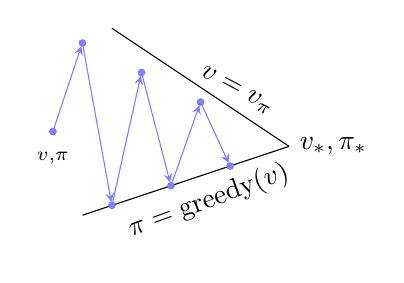
\begin{tikzpicture}[scale=3/4]
    \draw (-3, 2) -- (0, 0) node[above left = 3mm, rotate = -28] {$v = v_\pi$};  % y = -1/2x
    \draw (-3.5,-1.16666) -- (0, 0) node[below left, rotate=20] {$\pi =       \textrm{greedy}(v)$}; % y= 1/3*x
    \node at (0.75, 0) {$v_*, \pi_*$};
    \node[draw,circle,fill,scale=1/4,blue!50] (init) at (-4, 0.25) {};
    \node[below = 1mm of init] {$\scriptstyle v,\pi$};
    \node[draw,circle,fill,scale=1/4,blue!50] (one)  at (-3.5, 1.75) {};
    \node[draw,circle,fill,scale=1/4,blue!50] (two)  at (-3, -1) {};
    \node[draw,circle,fill,scale=1/4,blue!50] (three)at (-2.5, 1.25) {};
    \node[draw,circle,fill,scale=1/4,blue!50] (four) at (-2, -2/3) {};
    \node[draw,circle,fill,scale=1/4,blue!50] (five) at (-1.5, 0.75) {};
    \node[draw,circle,fill,scale=1/4,blue!50] (six)  at (-1, -1/3) {};
    \draw[-stealth,blue!50] (init) -- (one);
    \draw[-stealth,blue!50] (one) -- (two);
    \draw[-stealth,blue!50] (two) -- (three);
    \draw[-stealth,blue!50] (three) -- (four);
    \draw[-stealth,blue!50] (four) --(five);
    \draw[-stealth,blue!50] (five) -- (six);
  \end{tikzpicture}
\end{document}